\documentclass{beamer}
\usetheme[pageofpages=of,% String used between the current page and the
                         % total page count.
          bullet=circle,% Use circles instead of squares for bullets.
          titleline=true,% Show a line below the frame title.
          alternativetitlepage=true,% Use the fancy title page.
       %   titlepagelogo=logo-polito,% Logo for the first page.
       %   watermark=watermark-polito,% Watermark used in every page.
       %   watermarkheight=100px,% Height of the watermark.
       %   watermarkheightmult=4,% The watermark image is 4 times bigger
                                % than watermarkheight.
          ]{Torino}

\setbeamertemplate{footline}{
  \begin{beamercolorbox}[wd=\paperwidth,ht=1ex,dp=1ex]{footline}
    \vspace{5pt} \hspace{1em} \insertframenumber/\inserttotalframenumber
  \end{beamercolorbox}
}

\author{Brendon J. Brewer}
\title{STATS 331 -- Introduction to Bayesian Statistics}
\institute{The University of Auckland}
\date{}


\linespread{1.3}
\usepackage{minted}
\usepackage[utf8]{inputenc}
\usepackage{dsfont}
\newcommand{\given}{\,|\,}
\newcommand{\balpha}{\boldsymbol{\alpha}}
\newcommand{\bmu}{\boldsymbol{\mu}}


\begin{document}

\frame{\titlepage}

\begin{frame}
\begin{center}
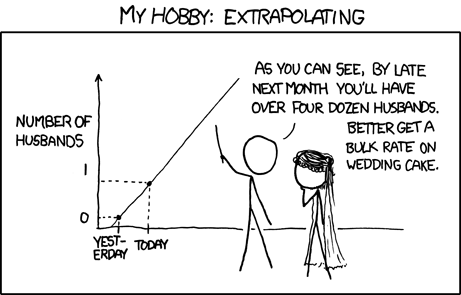
\includegraphics[width=0.6\textwidth]{images/extrapolating.png}

Credit: www.xkcd.com
\end{center}

\end{frame}


\begin{frame}
\Large

\begin{center}
Chi-Squared Test\footnote{Is not a test, and does not involve chi squared.}
\end{center}
\end{frame}


\begin{frame}
\frametitle{Motivating Example}

\begin{center}
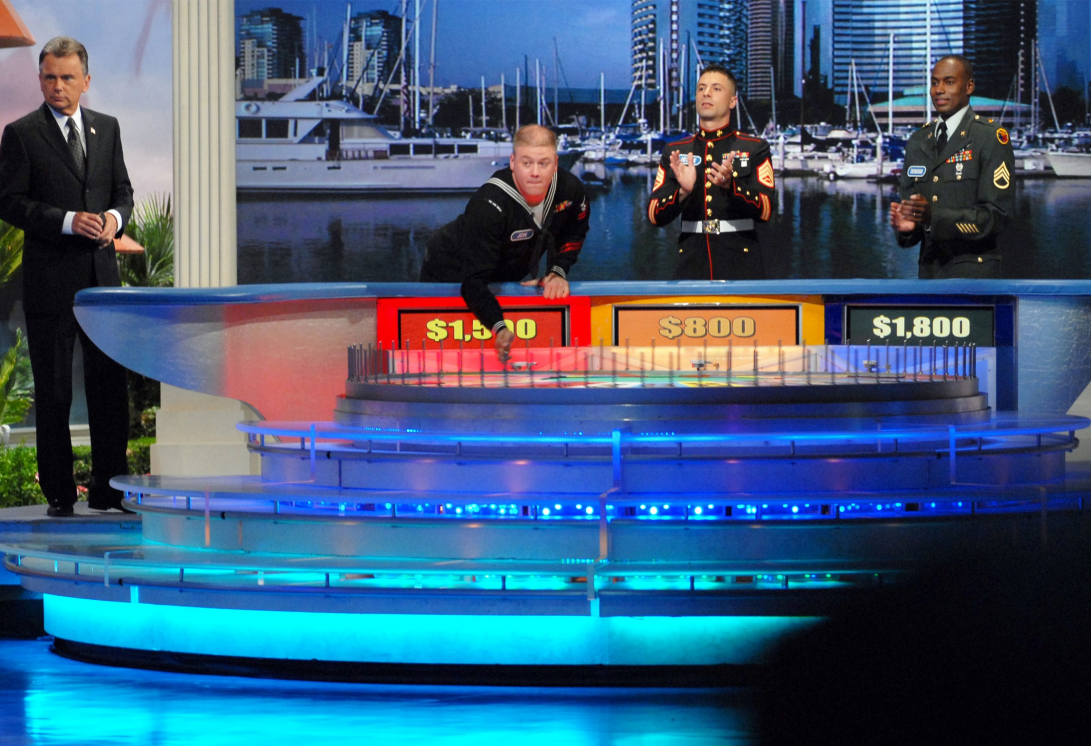
\includegraphics[width=0.6\textwidth]{images/wheel_of_fortune.png}

Source: Wikimedia Commons
\end{center}

\end{frame}


\begin{frame}
\frametitle{The Data}
The outcomes of $N=30$ Wheel of Fortune episodes:

\begin{center}
\begin{tabular}{|c|ccc|}
\hline
Position & 1 & 2 & 3 \\
\hline
Number of Wins $x$ & 8 & 9 & 13 \\
\hline 
\end{tabular}
\end{center}

\end{frame}

\begin{frame}
\frametitle{The Question}
We might wonder whether the following hypothesis is true:\\[0.5em]\pause

$H_0$: There is a 1/3 probability for each position to win each episode.

\end{frame}

\begin{frame}[fragile]
\frametitle{Classical Chi-Squared Test}
The classical `chi-squared test' is designed for this situation.
The test statistic is based on the difference between the observed counts
(8, 9, 13) and the expected counts under $H_0$ (10, 10, 10).
\pause
\begin{minted}{r}
> chisq.test(c(8, 9, 13))

	Chi-squared test for given probabilities

data:  c(8, 9, 13)
X-squared = 1.4, df = 2, p-value = 0.4966
\end{minted}

\end{frame}

\begin{frame}[fragile]
\frametitle{Classical Chi-Squared Test}
The main {\bf advantage} of the classical chi-squared test is that it is very
easy to carry out because it is already implemented in R.\\[0.5em]\pause

The main {\bf disadvantages} are:\pause
\begin{itemize}
\item It returns a p-value, not a posterior probability, and is subject to the
usual objections.\pause
\item It is based on an approximation that assumes that the number of counts
in each bin is high. Typically $\geq 5$ is preferred.
\end{itemize}

\end{frame}


\begin{frame}
\frametitle{Let's Make it Bayesian}
\begin{itemize}
\item Think of it as parameter estimation.\pause
\item There are $N$ trials and we will assume that, on each trial, the
probabilities for each `bin' are $(\theta_1, \theta_2, \theta_3)$.\pause
\item We will get the posterior distribution for the $\theta$ parameters
given the $x$ data (counts).\pause
\item This will involve two new distributions: the {\bf Dirichlet} for the
prior and the {\bf Multinomial} for the sampling distribution.
\end{itemize}

\end{frame}

\begin{frame}
\frametitle{From Binomial to Multinomial}

\begin{itemize}
\item Binomial situation: $N$ trials, success (with probability $\theta$)
or failure $(1-\theta)$ on each trial. We observe $x$ successes and $(N-x)$
failures, and the binomial distribution applies to $x$.\pause
\item Multinomial situation: $N$ trials, with bin probabilities
$\theta_1, \theta_2, ..., \theta_M$. We observe the counts in each bin,
$x_1, ..., x_M$.
\end{itemize}

\end{frame}

\begin{frame}
\frametitle{From Binomial to Multinomial}
The expression for the multinomial distribution is:

\begin{align}
p(x_1, ..., x_m \given \theta_1, ..., \theta_m)
    &= \frac{N!}{x_1!x_2!...x_M!}\theta_1^{x_1}\theta_2^{x_2}...\theta_M^{x_M}.
\end{align}
\pause

This gives the probability of obtaining $x_1$ outcomes in bin 1,
$x_2$ outcomes in bin 2, and so on, when the probabilities
of each bin on each trial are given by the $\theta$ parameters.

\end{frame}


\begin{frame}
\frametitle{Important Constraints}
We have important constraints on the parameters ($\theta$s) and the counts
($x$s):

\begin{align}
\theta_1 + \theta_2 + ... + \theta_M &= 1 \\
x_1 + x_2 + ... + x_M &= N.
\end{align}

\end{frame}


\begin{frame}
\frametitle{From Multinomial to Binomial}
If there are $M=2$ bins, and we call one `success' and the other `failure',
then the multinomial distribution becomes

\begin{align}
p(x_1, x_2 \given \theta_1, \theta_2)
    &= \frac{N!}{x_1!x_2!}\theta_1^{x_1}\theta_2^{x_2}.
\end{align}

which is an alternative way of writing the Binomial distribution

\begin{align}
p(x_1 \given \theta_1)
    &= \binom{N}{x_1}\theta_1^{x_1}(1 - \theta_1)^{N - x_1}.
\end{align}


\end{frame}


\begin{frame}[fragile]
\frametitle{Multinomial Distribution in JAGS}
The multinomial distribution in JAGS is easy to specify:
\begin{minted}{r}
x ~ dmulti(theta, N)
\end{minted}
\pause

This is very similar to \mintinline{r}{x ~ dbin(theta, N)} except that
\mintinline{r}{theta} is now a vector (the bin probabilities) and
\mintinline{r}{x} is also a vector (the counts in each bin).

\end{frame}


\begin{frame}[fragile]
\frametitle{Prior Distribution for the Bin Probabilities}
We need a prior for the bin probabilities $\theta_1, ..., \theta_M$.
We have the constraint $\sum_{i=1}^M \theta_i = 1$, which we haven't seen before.\pause

There is a useful distribution for this situation and it happens to be the
conjugate prior for the multinomial. It is called the {\bf Dirichlet distribution}. The expression is
\begin{align}
p(\theta_1, ..., \theta_M \given \alpha_1, ..., \alpha_M)
    &\propto \prod_{i=1}^M \theta_i^{\alpha_i - 1}.
\end{align}
\pause

There are hyperparameters called $\alpha$, one for each bin, and we will
see a little bit of what they do soon.

\end{frame}


\begin{frame}[fragile]
\frametitle{Dirichlet Special Case}
If we have $M=2$ bins the Dirichlet becomes a Beta distribution for the
probability of the first bin, with the probability of the second bin being
given deterministically by $\theta_2 = 1-\theta_1$.

\end{frame}


\begin{frame}[fragile]
\frametitle{Simplex}
The constraint that the $\theta$s all add up to 1 forms a `simplex'. It looks
like this:

\begin{center}
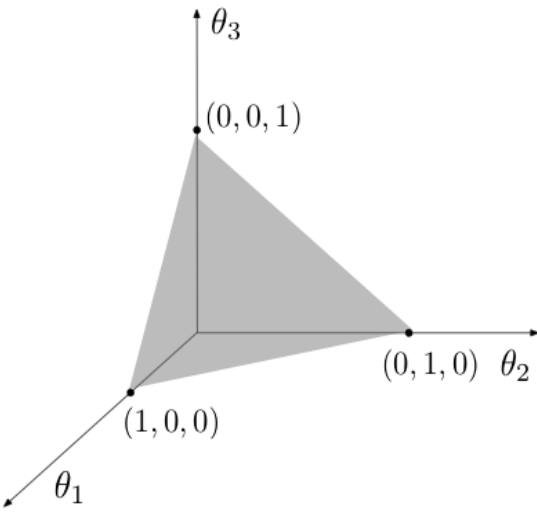
\includegraphics[width=0.45\textwidth]{images/simplex.png}

Source: theanalysisofdata.com
\end{center}

\end{frame}


\begin{frame}[fragile]
\frametitle{Role of the $\alpha$ Hyperparameters}
\begin{itemize}
\item The $\alpha$ parameters of the Dirichlet distribution control how similar
or different the $\theta$ (bin probabilities) are.\pause
\item We will use a common $\alpha$ value for all bins, which means we have no
prior information that any bin is more likely than any other.\pause
\item If $\alpha$ is low, there is a high prior probability that the $\theta$s
are very different from each other. Some bins hog a lot of the probability.\pause
\item If $\alpha$ is high, there is a lot of prior probability for the
$\theta$s to be similar to each other. Probability is divided close to equally.
\end{itemize}


\end{frame}


\begin{frame}[fragile]
\frametitle{Role of $\alpha$}
If $\alpha$ is low, the corners of the simplex are more plausible.
If $\alpha$ is high, the middle of the simplex is more plausible.
\end{frame}

\begin{frame}[fragile]
\frametitle{Dirichlet Prior in JAGS}
We can specify the Dirichlet prior easily, but we must have a vector of
\mintinline{r}{alpha}s set up first. For example:

\begin{minted}{r}
for(i in 1:3)
{
    alpha[i] <- 1
}
theta ~ ddirch(alpha)
\end{minted}
\pause

With all $\alpha$s set to 1, we have a uniform prior over the simplex.
\end{frame}

\begin{frame}[fragile]
\frametitle{Model 1}
\begin{minted}{r}
model
{
    for(i in 1:3)
    {
        alpha[i] <- 1
    }
    theta ~ ddirch(alpha)
    x ~ dmulti(theta, N)
}
\end{minted}
\end{frame}

\begin{frame}
\frametitle{Model 1 Results}
Let's run the model and look at:

\begin{itemize}
\item The posterior distribution for one of the $\theta$s.\pause
\item The posterior probability that \mintinline{r}{theta[3] > theta[2]}.\pause
\item {\bf Note}: We have given up on a precise $H_0$, like in our `one way ANOVA' model. The prior and posterior probabilities for the bin probabilities
being $(1/3, 1/3, 1/3)$ are zero.
\end{itemize}

\end{frame}


\begin{frame}[fragile]
\frametitle{Unknown Hyperparameters}
We do not have to assume that $\alpha=1$. We could let it be unknown.
\footnotesize
\begin{minted}{r}
model
{
    log_a ~ dunif(-1, 10)
    for(i in 1:3)
    {
        alpha[i] <- exp(log_a)
    }
    theta ~ ddirch(alpha)
    x ~ dmulti(theta, N)
}
\end{minted}

\end{frame}


\begin{frame}[fragile]
\frametitle{Model 1 Results}
Let's run the model and look at:

\begin{itemize}
\item The posterior distribution for one of the $\theta$s.\pause
\item The posterior probability that \mintinline{r}{theta[3] > theta[2]}.\pause
\item The posterior distribution for \mintinline{r}{log_a} (whose prior was
uniform). This will tell us whether the bins are really similar (high values
of \mintinline{r}{log_a}) or very different
(low values of \mintinline{r}{log_a}).
\end{itemize}

\end{frame}


\begin{frame}[fragile]
\frametitle{Conclusion}
This was just another common data analysis scenario, but allowed us to see two
important distributions, one of which is the conjugate prior for the other.\pause

For pragmatic reasons (inability to calculate marginal likelihoods in STATS 331) we followed
our usual pattern of replacing the hypothesis test with parameter estimation,
where some of the parameter space is similar to $H_0$.
\end{frame}


\end{document}

